\chapter{Projekt GUI}
\label{cha:projekt-gui}

Interfejs użytkownika systemu OSK-Manager został zaprojektowany jako aplikacja webowa dostępna z poziomu przeglądarki. Głównym założeniem GUI jest szybki dostęp do najważniejszych obszarów pracy szkoły jazdy: kursantów, instruktorów, kursów, pojazdów, harmonogramu, płatności i ocen.

\section{Założenia interfejsu}
\label{sec:zalozenia-gui}

Aplikacja wykorzystuje układ panelowy. Po zalogowaniu użytkownik widzi obszar roboczy z nawigacją boczną, górnym paskiem oraz właściwą treścią strony. Nawigacja zależy od roli użytkownika. Manager otrzymuje dostęp do funkcji administracyjnych szkoły, instruktor do własnego harmonogramu i ocen, natomiast kursant do swoich kursów, lekcji, płatności i możliwości rezerwacji terminu.

Widoki systemu powinny być czytelne zarówno na komputerze, jak i na urządzeniach mobilnych. Listy i tabele są używane tam, gdzie użytkownik porównuje wiele rekordów, na przykład kursantów, instruktorów lub pojazdy. Kalendarze i siatki czasu są używane w obszarach harmonogramu. Formularze są dzielone na logiczne sekcje, aby ułatwić wprowadzanie danych.

\section{Widok logowania}
\label{sec:gui-logowanie}

Widok logowania umożliwia użytkownikowi podanie adresu e-mail oraz hasła. Formularz sprawdza, czy wymagane pola zostały uzupełnione, a następnie wysyła dane do mechanizmu autoryzacji. Po poprawnym zalogowaniu użytkownik zostaje przekierowany do aplikacji. Jeżeli użytkownik był już zalogowany, system może przekierować go bezpośrednio do właściwego widoku.

W środowisku demonstracyjnym aplikacja może udostępniać przyciski uzupełniające pola przykładowymi danymi. Mechanizm ten ma charakter pomocniczy i nie zastępuje właściwego procesu logowania.

\begin{figure}[H]
\centering
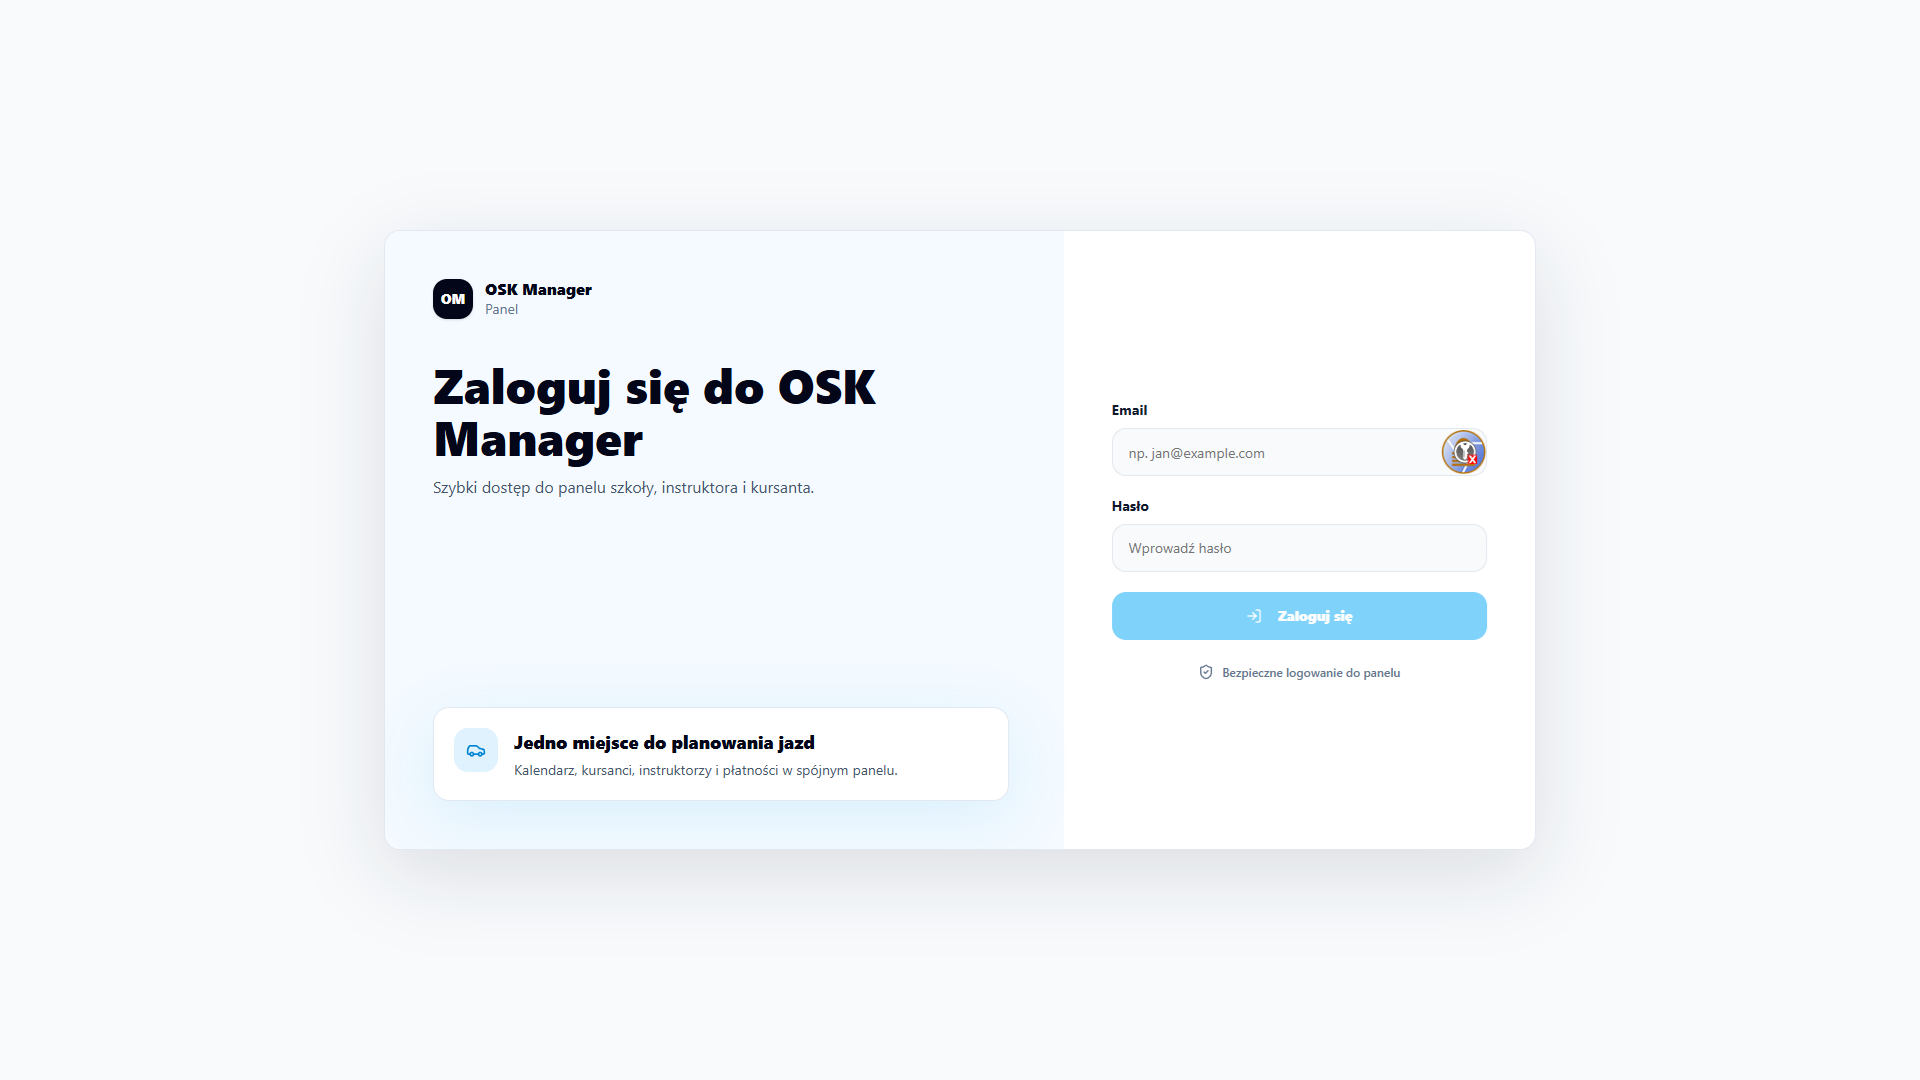
\includegraphics[width=\textwidth]{figures/generated/gui-login.png}
\caption{Widok logowania do systemu OSK-Manager}
\label{fig:gui-logowanie}
\wsizsource{Opracowanie własne}
\end{figure}
\section{Dashboard}
\label{sec:gui-dashboard}

Dashboard jest pierwszym widokiem po zalogowaniu. Dla managera prezentuje kontekst domyślnego ośrodka szkolenia kierowców oraz skrót do harmonogramu i dostępności instruktorów. Jeżeli manager nie ma ustawionego domyślnego OSK, aplikacja prowadzi go do konfiguracji ośrodka.

Dla kursanta i instruktora dashboard pełni funkcję widoku startowego. Może prezentować przypisane szkoły, najważniejsze odnośniki oraz informacje potrzebne do przejścia do kursów, lekcji albo harmonogramu.

\begin{figure}[H]
\centering
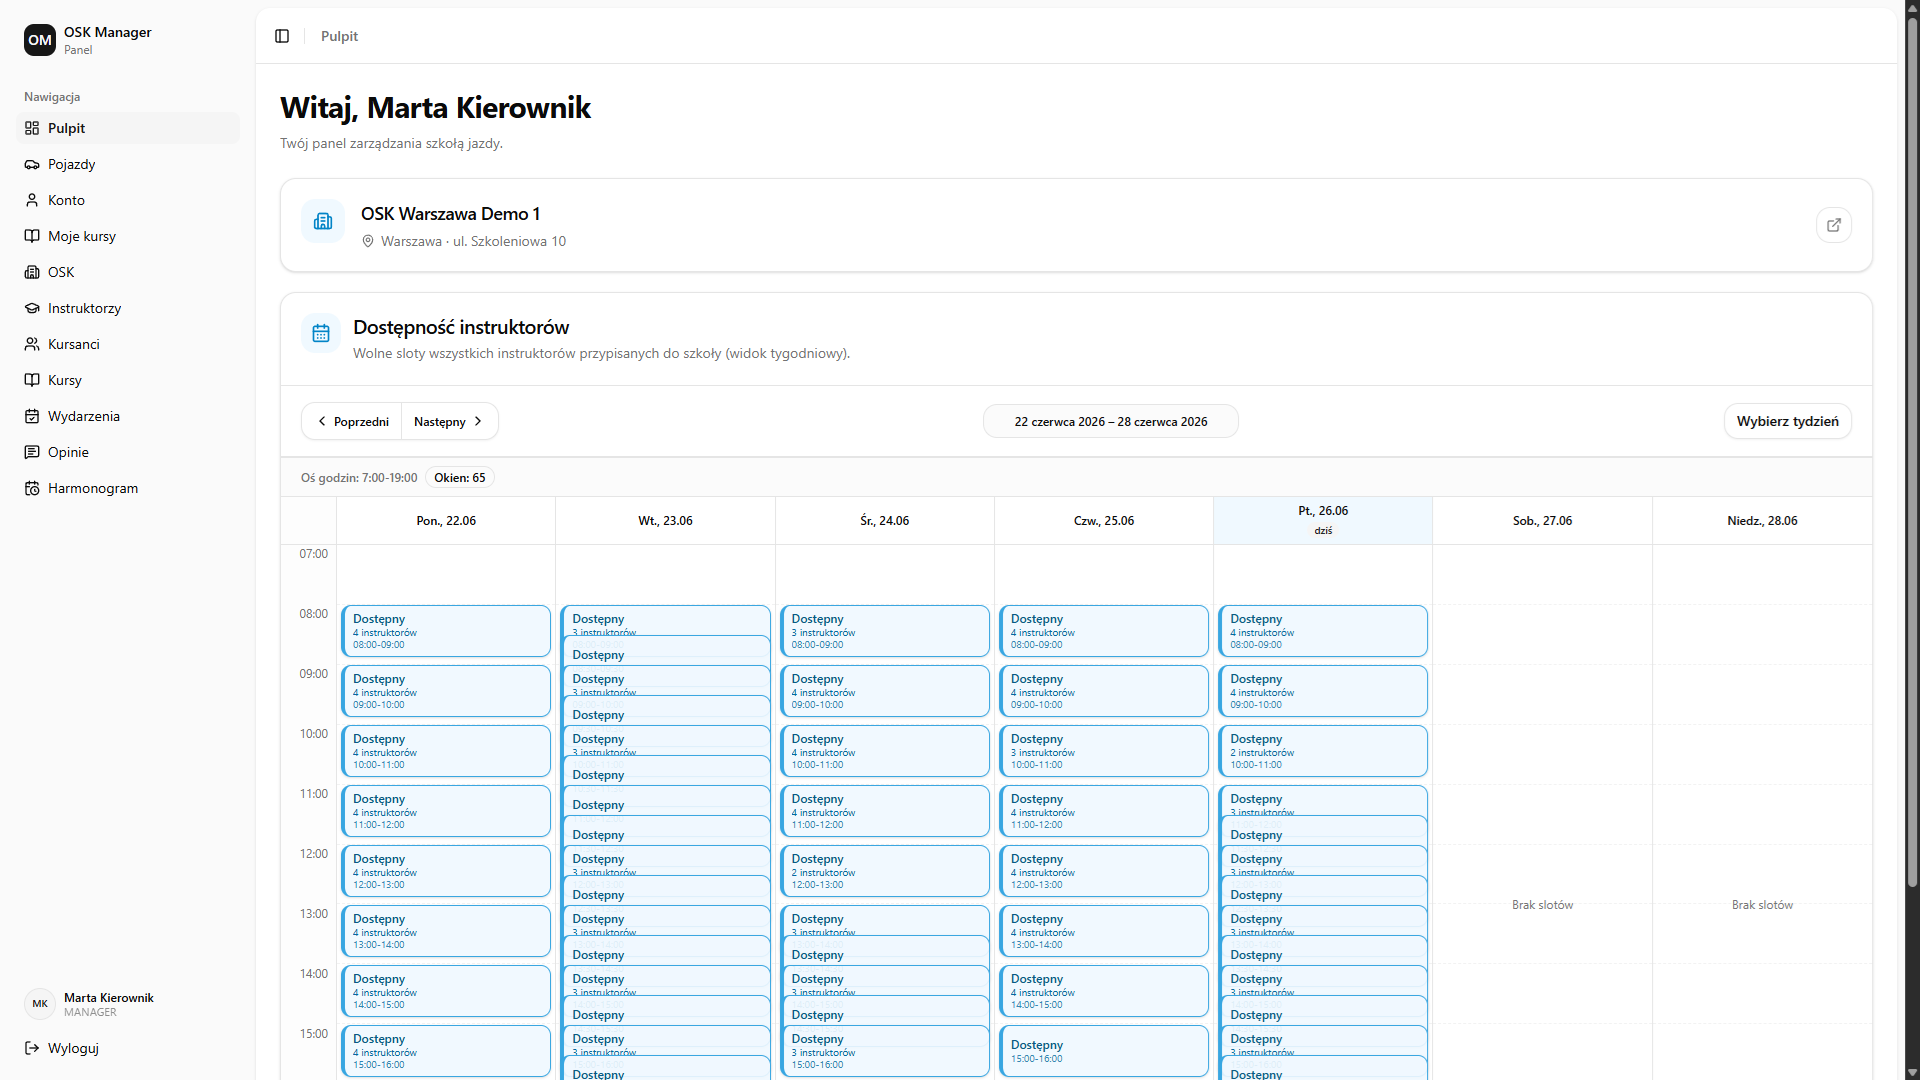
\includegraphics[width=\textwidth]{figures/generated/gui-dashboard.png}
\caption{Dashboard managera z dostępnością instruktorów}
\label{fig:gui-dashboard}
\wsizsource{Opracowanie własne}
\end{figure}
\section{Panel managera}
\label{sec:gui-panel-managera}

Panel managera obejmuje widoki przeznaczone do zarządzania szkołą jazdy. Najważniejsze obszary to:
\begin{itemize}
    \item lista i szczegóły kursantów,
    \item lista i szczegóły instruktorów,
    \item zarządzanie ośrodkami szkolenia kierowców,
    \item zarządzanie kursami,
    \item zarządzanie pojazdami,
    \item harmonogram szkoły,
    \item edycja lekcji i wydarzeń,
    \item przegląd ocen lekcji.
\end{itemize}

Widok kursantów pozwala przeglądać listę osób przypisanych do szkoły, filtrować dane, dodać kursanta oraz przypisać go do kursu. Szczegóły kursanta obejmują dane profilu, status procesu szkolenia, notatki, harmonogram lekcji, płatności i kursy.

Widok instruktorów pozwala dodawać instruktorów, przeglądać ich dane, kwalifikacje, dostępność, harmonogram i oceny. Manager może przejść do edycji dostępności, sprawdzić tygodniowy grafik oraz zarządzać blokadami czasu.

Widok pojazdów pozwala przeglądać flotę szkoły, dodawać pojazdy, edytować ich dane, oznaczać status dostępności i przechowywać podstawowe informacje eksploatacyjne, takie jak numer rejestracyjny, marka, model, przebieg, przegląd i ubezpieczenie.

Widok harmonogramu prezentuje zajęcia szkoły w ujęciu czasowym. Manager może analizować obłożenie instruktorów, sprawdzać zaplanowane lekcje oraz przechodzić do edycji wydarzeń. Harmonogram jest jednym z kluczowych widoków systemu, ponieważ łączy dane kursantów, instruktorów, pojazdów i kursów.

\begin{figure}[H]
\centering
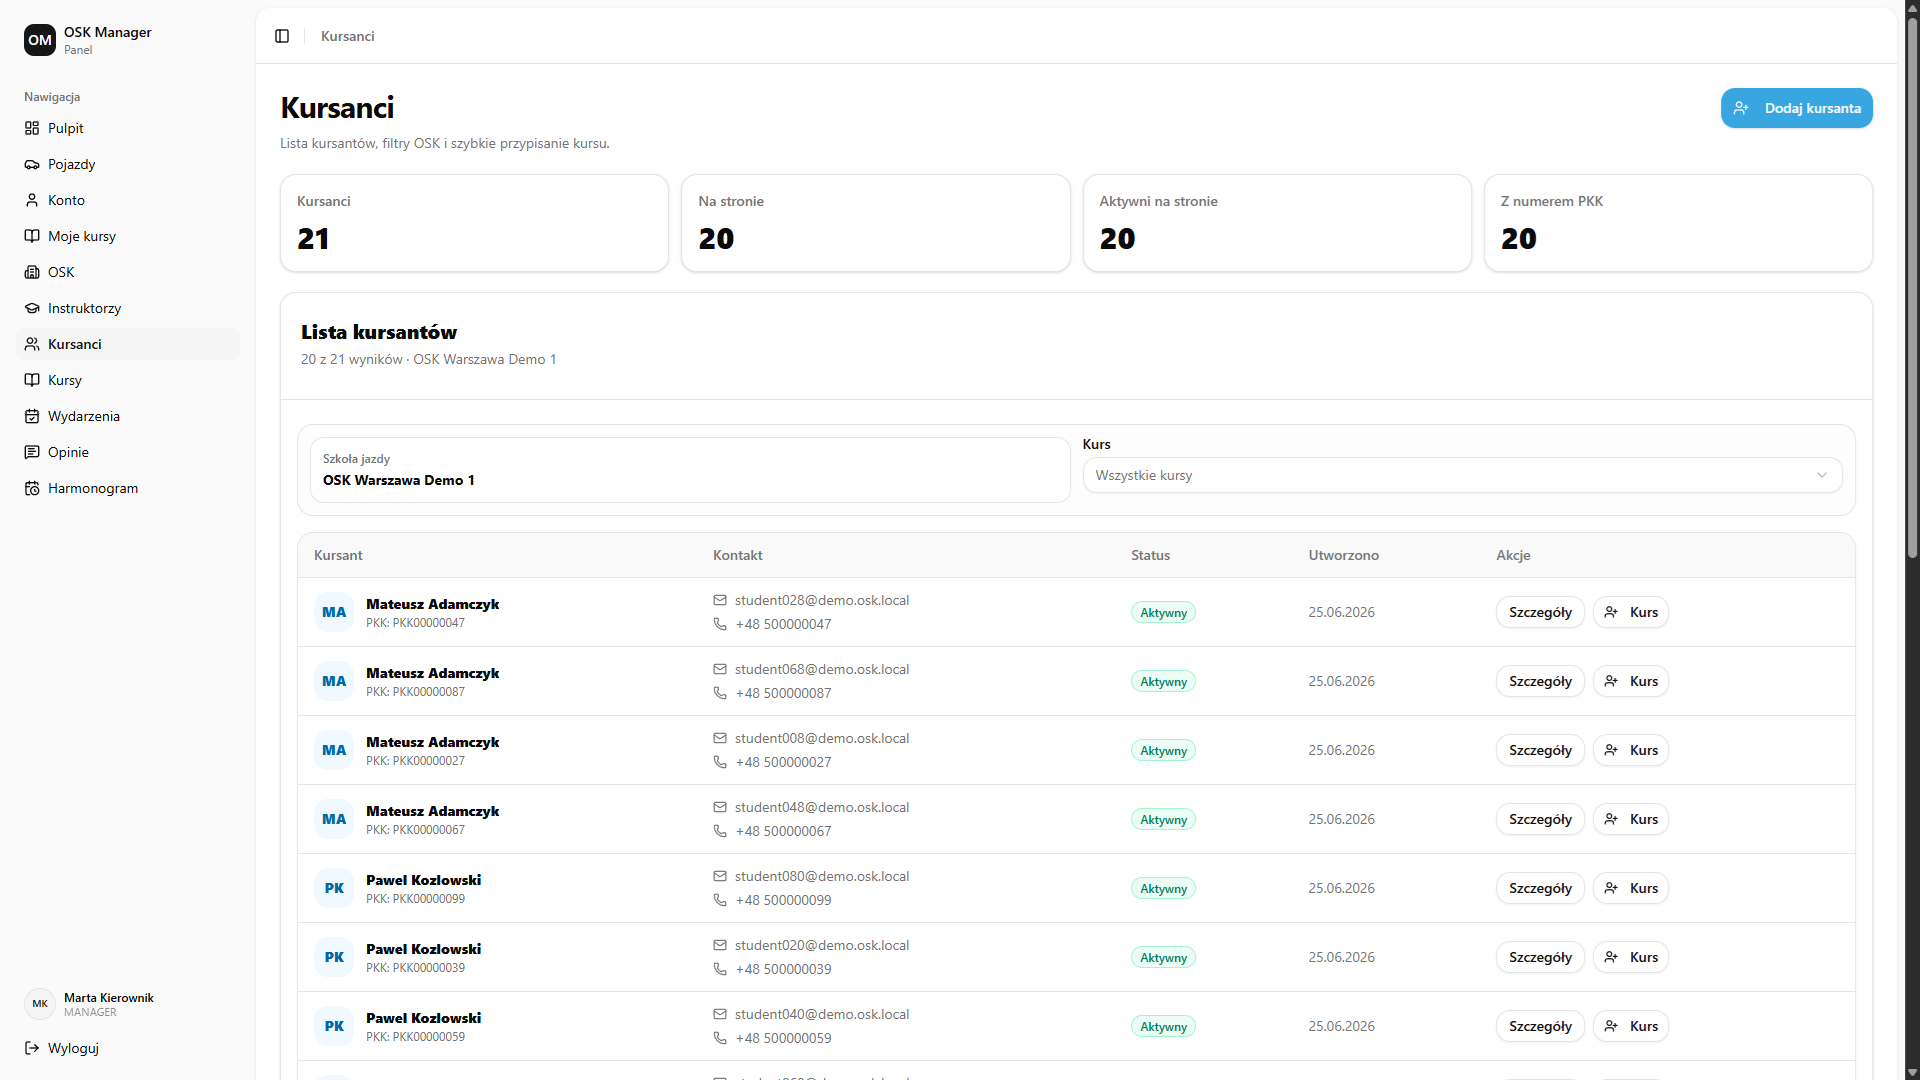
\includegraphics[width=\textwidth]{figures/generated/gui-students-list.png}
\caption{Widok listy kursantów w panelu managera}
\label{fig:gui-lista-kursantow}
\wsizsource{Opracowanie własne}
\end{figure}

\begin{figure}[H]
\centering
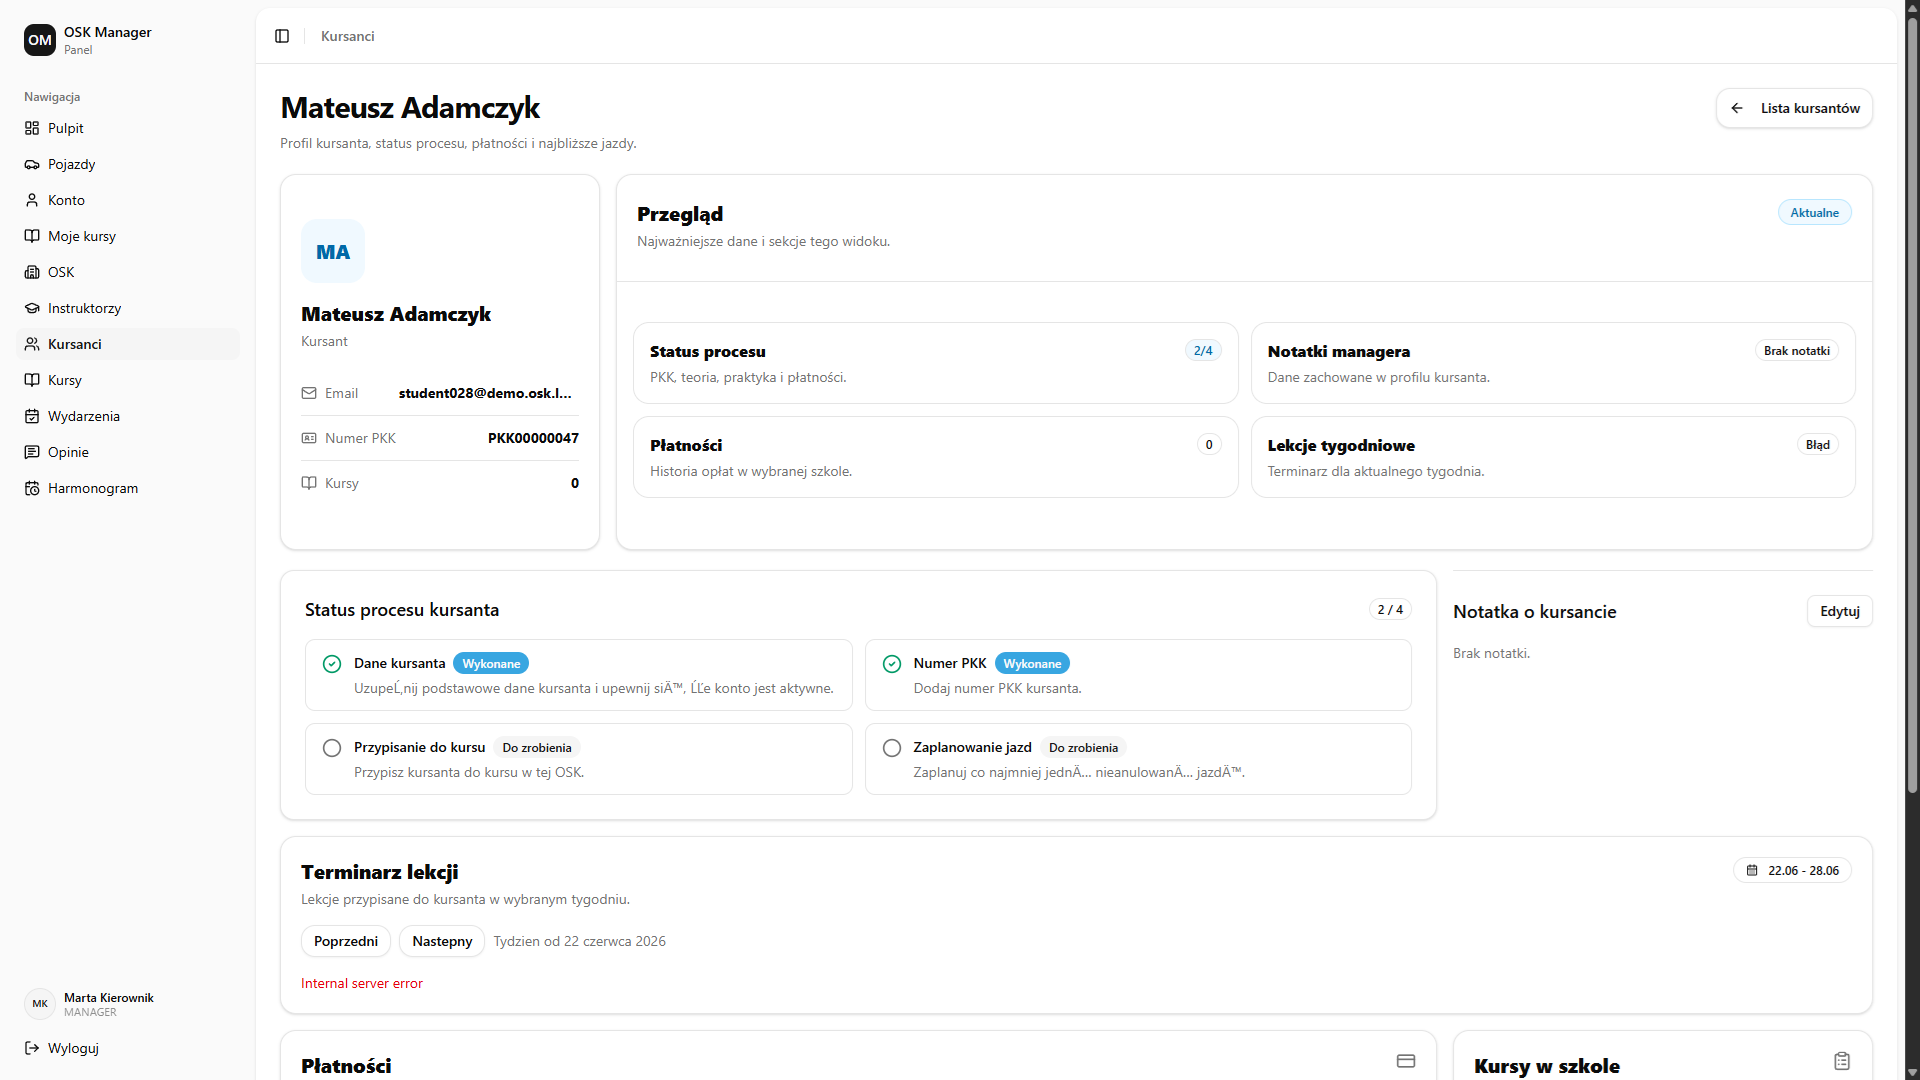
\includegraphics[width=\textwidth]{figures/generated/gui-student-details.png}
\caption{Widok szczegółów kursanta w panelu managera}
\label{fig:gui-szczegoly-kursanta}
\wsizsource{Opracowanie własne}
\end{figure}

\begin{figure}[H]
\centering
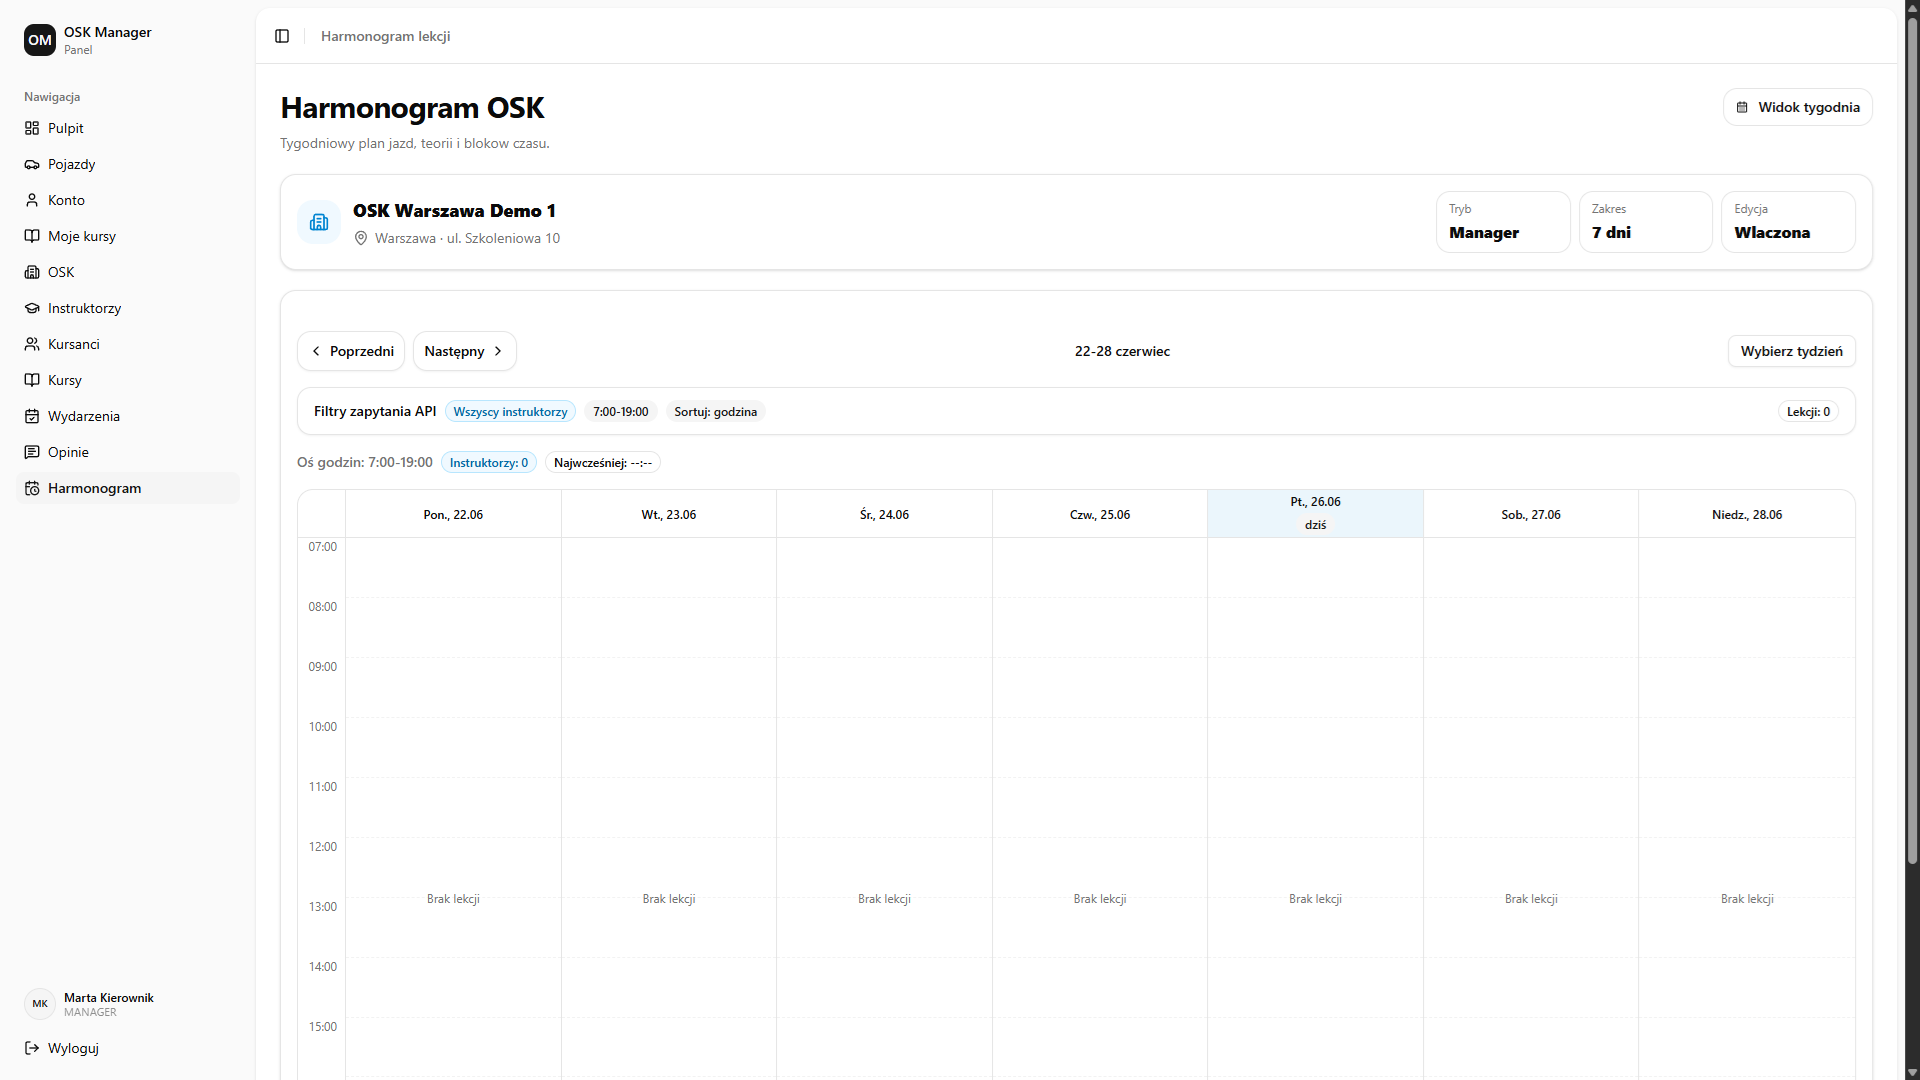
\includegraphics[width=\textwidth]{figures/generated/gui-schedule.png}
\caption{Widok harmonogramu OSK w panelu managera}
\label{fig:gui-harmonogram}
\wsizsource{Opracowanie własne}
\end{figure}
\section{Widoki kursanta}
\label{sec:gui-kursant}

Kursant korzysta z widoków związanych z własnym szkoleniem. Może przeglądać swoje kursy, zaplanowane lekcje, płatności oraz oceny. Widok rezerwacji lekcji pozwala wybrać kurs, tydzień oraz dostępny termin, a następnie zapisać lekcję, jeżeli spełnione są warunki dostępności.

W widoku lekcji kursant może sprawdzić nadchodzące i zakończone zajęcia. Dla zakończonych lekcji praktycznych dostępny jest mechanizm wystawienia oceny. System blokuje ocenę lekcji, jeżeli nie została zakończona, nie jest lekcją praktyczną albo została już wcześniej oceniona.

\section{Widoki instruktora}
\label{sec:gui-instruktor}

Instruktor korzysta przede wszystkim z widoków harmonogramu oraz ocen. Może sprawdzić swoje lekcje i wydarzenia oraz zobaczyć opinie wystawione przez kursantów. Część widoków jest współdzielona z kursantem, ale prezentowane dane są filtrowane zgodnie z rolą użytkownika.

\section{Wspólne elementy interfejsu}
\label{sec:gui-wspolne-elementy}

W wielu widokach powtarzają się te same wzorce interfejsu. Listy danych posiadają stany ładowania, puste stany oraz komunikaty błędów. Formularze pokazują walidację i blokują zapis w trakcie wysyłania danych. Dialogi służą do tworzenia, edycji lub potwierdzania operacji, na przykład usunięcia rekordu albo anulowania lekcji.

System wykorzystuje oznaczenia statusów w formie etykiet, przyciski akcji, selektory, filtry, pola daty i czasu oraz komponenty kalendarza. Dzięki temu użytkownik może wykonywać podobne operacje w podobny sposób w różnych częściach aplikacji.
